\documentclass[12pt]{toptesi}
\usepackage{amsmath}
\usepackage{booktabs}
\usepackage{color}
\usepackage{amssymb}    % e.g., for \mathbb{}
\usepackage[]{units}
\usepackage{tikz}
\usetikzlibrary{arrows,positioning}
\usetikzlibrary{calc} % for manimulation of coordinates
\usetikzlibrary{matrix}
\usetikzlibrary{circuits.logic.US,circuits.logic.IEC}
\usetikzlibrary{positioning}
\tikzstyle{cs}=[circle,fill=black,minimum size=3pt,inner sep=0pt]
\tikzset{
  -|-/.style={
    to path={
      (\tikztostart) -| ([xshift=-#1]$(\tikztotarget)$) |- (\tikztotarget)
      \tikztonodes
    }
  },
  -|-/.default=5pt,
	--|-/.style={
    to path={
      (\tikztostart) -- ++(right:#1) |- (\tikztotarget)
      \tikztonodes
    }
  },
  --|-/.default=3pt,
}
\newcommand\bx{\mathbf{x}}
\newtheorem{definition}{Definition}
\newtheorem{theorem}{Theorem}
\newtheorem{proof}{Proof}
\newtheorem{example}{Example}

\begin{document}
\english
\begin{frontespizio*}
    \ateneo{Politecnico di Torino}
    \logosede{logo_poli.png}
    \StrutturaDidattica{Dipartimento di }
    \struttura{Elettronica e Telecommunicazioni}
    \corsodilaurea{Ingegneria Elettronica}
    \TesiDiLaurea{Tesi di Laurea Magistrale}
    \titolo[]{Boh}
    \relatore{Luciano Lavagno}
    \candidato{Daniel Rodas Bautista \IDN s219976}
    \sedutadilaurea{Luglio 2016}
\end{frontespizio*}

\tableofcontents
\listoffigures
\listoftables


\chapter*{Acknowledgments}
%Emanuel, Lavagno, Bo, Satish, Sara, iRISC, 

\chapter{Introduction}

EDA for Reliability and low power.
Different methodologies are being analysed to improve the reliability and power consumption of a circuit:
-Use of error correcting techniques, from communication theory, in digital design.
-Decomposition of the circuit into Reed-Muller form.
-Decomposition into cones, increasing redundancy and minimising error propagation throughout the circuit. 

\chapter{Motivations}
    \section{AND-XOR network synthesis}
Logic synthesis for low power and more recently reliability is a widely studied subject with many tools being developed throughout industry and academia. State of the art synthesis flows aim at optimizing performance or area or power of a given logic function. During the synthesis process, the redundancy which is inherently captured in its truth table is reduced or indeed removed hence impacting the reliability of the circuit. One can conclude that the most reliable function is represented by the sum of constituent minterms (or sum of products SOP form). However, this un-optimized function leads to a very large area/delay/power overhead given its exponential number of minterms.  Fault tolerant techniques for improving  reliability of digital circuitry have been of interest from long time. Von Neumann \cite{Neumann56} firstly introduced a classification of the error types and proposed some solutions as early as 1956. Important work to cross the field of circuit design with the knowledge of error correction theory has been done by Taylor \cite{Taylor68a, Taylor68b} that used Low Density Parity Check (LDPC) codes to build fault tolerant architectures for reliable systems.

From a gate level perspective, there are two methodologies to improve the reliability of a given circuit while maintaining a minimal overhead. The first method as already presented in \cite{Grandhi15}, is reliability optimization using combinatorial methods and graph manipulations. It was shown that these lead to relatively modest reliability improvements, but with minimal area/delay/power overhead \cite{Grandhi15}. 
While the reliability is improved, the circuit is still not fault-tolerant. In this methodology, the number of outputs (or function associated truth table size) is not increased. Instead, the graph is transformed through a sequence of application of a number of rules in order to increase its reliability. A second method of adding redundancy is by modifying the size of the function associated truth table. 

In \cite{D5.2, ETS}, a new methodology called Code Prediction Encoding (CPE) was introduced with the view of extending the logic network with a parity network, hence increasing the number of outputs of the circuit. The focus of this approach is not on changing the combinational logic but on augmenting it. It enables the retrieval of the correct output even if errors have occurred. The process carries remembrance with the process of adding redundancy to the transmitted message in a communication system. It exploits the afferent topology of the original circuit, which is expanded by embedding an Error Correcting Code (ECC) into its logical functionality. 

Any code could be used, hence the generic nature of the technique. This method was successfully applied to improve the reliability of XOR-only logic networks (or linear circuits in our concept) in the context of LDPC encoding 
%[ICC]. 
\cite{ICC}. 
However, the majority of circuits in practice are non-linear in nature as they are built with arbitrary logic gates and hence they are less amenable for a CPE technique as remarked in \cite{D5.2}. 
Following the rationale of CPE approach, this paper summarizes relevant knowledge regarding the separation of a combinatorial circuit into a linear and a non-linear part. The linear part can be then used in context of CPE. The application of recently published ideas of the vectorial bi-decomposition \cite{S_VBD_LF_RM_2015} leads to a partition of circuit parts that contains either only non-linear AND-gates or only linear EXOR-gates. This is particularly interesting as it is known that AND-XOR network results in much better realization and requires fewer product terms than more classical AND-OR realization. 
 
We show that using our decomposition methods, one can derive the Reed-Muller form of a circuit which is known as a hard problem.
\cite{Knysh11}
Another contribution of this work is the quantification of the efficiency of linearization by introducing the notion of degree of linearization. The contributions are outlined on adders of varying size.

Adders are some of the most used non-linear logic functions in practice and numerous architectures were proposed to implement them. We show that even in the case of the symmetric carry function, for which no strong bi-decomposition exists \cite{BDS_NDM_MCD_EDAC_1991,MSP_ABD_LF_DAC_2001}, a decomposition into a linear output-part and a non-linear input part could be designed.

We apply the described decomposition at bit level, block level and unit level on an adder architecture and analyze the results in terms of area, delay, power on two technologies, namely ASIC and FPGA.

\section{CPE}

\chapter{Synthesis for Reliability by Bi-Decomposition}

%abstract from paper: A method for synthesizing adders in multi-level AND-XOR form is presented with different levels of granularity. This uses a vectorial decomposition methodology applied to adders. We show that the Reed-Muller form of an adder can be derived using our methodology. Furthermore, we give some insights into the degree of linearity for our adders. Finally, we present some results of implementations on ASIC and FPGA technologies. Results show that it is possible to decompose the netlist of an adder into a AND-network and XOR-network. This is a first step into further study for reliability optimization by embedding linear codes into the netlist of Boolean circuits. 

\section{Synthesis for Reliability}

The application of the CPE approach requires that the circuit structure is split into a linear and a non-linear part. Therefore we explore synthesis methods that find such a separated structure. Figure \ref{fig:dec_arch} shows the needed architecture of the circuit.


\begin{figure}
	\centering
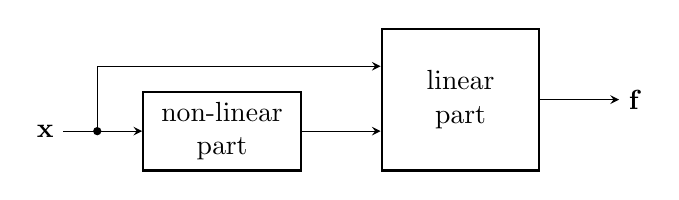
\begin{tikzpicture}[>=stealth]
\node[draw, thick, text width=17mm, text centered, minimum width = 20mm, minimum height = 10mm] (nlp) {non-linear part};
\node[draw, thick, text width=15mm, text centered, minimum width = 20mm, minimum height = 18mm, right=10mm of nlp, yshift= 4mm] (lp) {linear part};
\node[left=10mm of nlp] (x) {$\bx$};
\node[right=10mm of lp] (f) {$\mathbf{f}$};
\node[cs, right=6mm of x.center] (xp) {};
\node[above = 3mm of lp.west] (xlp) {};
\draw[->] (x) -- (nlp.west);
\draw[->] (lp.east) -- (f);
\draw[->] (nlp.east) -- (lp.west |- nlp.east);
\draw[->] (xp.center) |- (xlp.center);
\end{tikzpicture}		
	\caption{Preferred architecture for circuits with a high reliability.}
	\label{fig:dec_arch}
\end{figure}

\subsection{Linearity with Regard to a Variable}
\label{subsec:lin_wrt_v}
The Linearity is a property of a Boolean function which is defined regarding each variable. 

\begin{definition}[Linearity]
A Boolean function $f(x_i,\bx_0)$ is linear with regard to the variable $x_i$ if and only if
\begin{equation}
\frac{\partial f(x_i,\bx_0)}{\partial x_i} = 1~.
\label{equ:lin_xi}
\end{equation}
\end{definition}

If the Boolean function $f(x_i,\bx_0)$ satisfies \eqref{equ:lin_xi} this function can be expressed by
\begin{equation}
f(x_i,\bx_0)=x_i \oplus g(\bx_0)
\label{equ:lin_sep_xi}
\end{equation}
The function $g(\bx_0)$ can be calculated by
\begin{equation}
g(\bx_0) = \max_{x_i} \left(x_i \oplus f(x_i,\bx_0)\right)~,
\label{equ:g_x0}
\end{equation}
using the derivative operation \textit{single maximum} of the BDC \cite{SP_BDC_2010}. The function $g(\bx_0)$ is independent of the variable $x_i$. The independence of a variable $x_i$ is also a property of a Boolean function.

\begin{definition}[Independence]
A Boolean function $f(x_i,\bx_0)$ is independent of the variable $x_i$ if and only if
\begin{equation}
\frac{\partial f(x_i,\bx_0)}{\partial x_i} = 0~.
\label{equ:indep_xi}
\end{equation}
\end{definition}

\begin{example}[Linear separation of $x_i$]
%[from the sum function $f_s(x_i, y_i, c_{i-1})$ of an adder cell]
The sum function $f_{s_i}(x_i, y_i, c_{i-1})$ of the adder cell $i$ is defined by
\begin{equation}
f_{s_i}(x_i,y_i,c_{i-1}) = 
\overline{x}_i\, \overline{y}_i\, c_{i-1} \vee
\overline{x}_i\, y_i\, \overline{c}_{i-1} \vee
x_i\, \overline{y}_i\, \overline{c}_{i-1} \vee
x_i\, y_i\, c_{i-1} ~.
\label{equ:fsi}
\end{equation}
This function satisfies the condition \eqref{equ:lin_sep_xi} of the linearity with regard to the variable $x_i$
\begin{equation}
\frac{\partial f_{s_i}(x_i,y_i,c_{i-1}) }{\partial x_i} = 1~,
\label{equ:fsi_lin_xi}
\end{equation}
which follows form the definition of the derivative
\begin{equation}
\frac{\partial f(x_i,\bx_0)}{\partial x_i} = f(x_i=0,\bx_0) \oplus f(x_i=1,\bx_0)~
\label{equ:sder_def_xi}
\end{equation}
applied to \eqref{equ:fsi}:
\begin{align*}
	\frac{\partial f_{s_i}(x_i,y_i,c_{i-1}) }{\partial x_i} 
	&= 
(
\overline{y}_i\, c_{i-1} \vee
y_i\, \overline{c}_{i-1} \vee
\overline{y}_i\, \overline{c}_{i-1})
\oplus
(y_i\, c_{i-1})\\
	&= 
\overline{y}_i \oplus
y_i\, \\
	&= 1~.
\end{align*}
Using the definition of the maximum with regard to $x_i$
\begin{equation}
\max_{x_i} f(x_i,\bx_0) = f(x_i=0,\bx_0) \vee f(x_i=1,\bx_0)~
\label{equ:smax_def_xi}
\end{equation}
the function $g(y_i,c_{i-1})$ and can be calculated based on \eqref{equ:g_x0}:
\begin{align*}
	g_{s_i}(y_i,c_{i-1}) &= \max_{x_i} \left(x_i \oplus f_{s_i}(x_i,y_i,c_{i-1}) \right)\\
	&= \left(0 \oplus 
	(
	\overline{y}_i\, c_{i-1} \vee
y_i\, \overline{c}_{i-1}  
)
	\right)
\vee
\left(1 \oplus 
	(
\overline{y}_i\, \overline{c}_{i-1} \vee
y_i\, c_{i-1} 
)
	\right)
	\\
		&= 
	\overline{y}_i\, c_{i-1} \vee
y_i\, \overline{c}_{i-1}~. 
\end{align*}
\begin{figure}[b]
	\centering
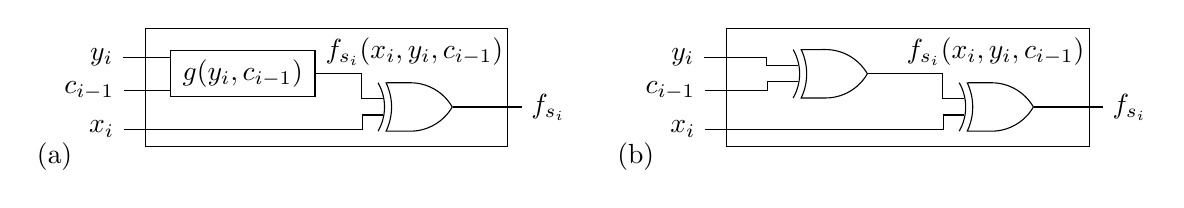
\begin{tikzpicture}[circuit logic US,
block/.style={rectangle,draw,
text width=1.6cm,
text centered,font=\sffamily,anchor=center},
]	
\begin{scope}%[yshift=60]
\node (g) [block,xshift=18, yshift=12] {$g(y_i,c_{i-1})$};
\node (xa)[xshift=-33, yshift=18] {$y_i$};
\node (xc)[xshift=-37.5, yshift=06] {$c_{i-1}$};
\node (xb)[xshift=-33, yshift=-8] {$x_i$};
\draw (-0.6,-0.5) -- (4,-0.5) -- (4,1) -- (-0.6,1) -- cycle;
\node (f) [xshift=80, yshift=20] {$f_{s_i}(x_i,y_i,c_{i-1})$};
\node [xor gate, xshift=80] (gxo) {}; 
\node (y)[right of=gxo, xshift=20] {$f_{s_i}$};
\draw (gxo.output) -- (y.west);
\draw (xa.east) -- (xa.east-|g.west);
\draw (xc.east) -- (xc.east-|g.west);
\draw (xb.east) to[--|-={30.3mm}] (gxo.input 2);
\draw (g.east) to[--|-={5.8mm}] (gxo.input 1);
\node (a) [xshift=-50, yshift=-18] {(a)};
\end{scope}
\begin{scope}[xshift=210]
%\node (g) [block,xshift=20, yshift=12] {$g(y_i,c_{i-1})$};
\node (xa)[xshift=-33, yshift=18] {$y_i$};
\node (xc)[xshift=-37.5, yshift=06] {$c_{i-1}$};
\node (xb)[xshift=-33, yshift=-8] {$x_i$};
\draw (-0.6,-0.5) -- (4,-0.5) -- (4,1) -- (-0.6,1) -- cycle;
\node (f) [xshift=80, yshift=20] {$f_{s_i}(x_i,y_i,c_{i-1})$};
\node [xor gate, xshift=80] (gxo1) {}; 
\node [xor gate, xshift=20, yshift=12] (gxo2) {}; 
\node (y)[right of=gxo1, xshift=20] {$f_{s_i}$};
\draw (gxo1.output) -- (y.west);
\draw (xa.east) to[--|-={8.0mm}] (gxo2.input 1);
\draw (xc.east) to[--|-={8.0mm}] (gxo2.input 2);
\draw (xb.east) to[--|-={30.3mm}] (gxo1.input 2);
\draw (gxo2.output) to[--|-={9.5mm}] (gxo1.input 1);
\node (a) [xshift=-50, yshift=-18] {(b)};
\end{scope}
\end{tikzpicture}
	\caption{Separation of a variable using EXOR gates: (a) with regard to $x_i$, (b) consecutively with regard to $x_i$ and $c_{i-1}$
	}
	\label{fig:lin_sep_xi}
\end{figure}
Figure \ref{fig:lin_sep_xi} (a) shows the circuit structure created by this linear separation of the variable $x_i$.

The function $g(y_i,c_{i-1})$ is linear with regard to both the variables $c_{i-i}$ and $y_i$. Hence, 
	\[
	g(y_i,c_{i-1}) = y_i \oplus c_{i-1}
\]
and the function $f_{s_i}(x_i,y_i,c_{i-1})$ is completely linear 
	\[
	g(y_i,c_{i-1}) = x_i \oplus y_i \oplus c_{i-1}~.
\]
Figure \ref{fig:lin_sep_xi} (b) shows the circuit structure created by two linear separations of a single variable using two EXOR-gates.
\end{example}


\subsection{Degree of Linearity}

The derivative with regard to the variables $x_i$ is a Boolean function for which the extreme values specify either the linearity
 %\eqref{equ:lin_xi} 
by the value 1 or the independence 
%\eqref{equ:indep_xi} 
by the value 0. 

The single derivative itself is independent of $x_i$:
\begin{equation}
\frac{\partial }{\partial x_i} \left(\frac{\partial f(x_i,\bx_0)}{\partial x_i} \right)= 0~.
\label{equ:sder_indep_xi}
\end{equation}

The number of values 1 of the derivative with regard to the variable $x_i$ is a measure for the degree of the linearity. 

\begin{definition}[Degree of Linearity]
A Boolean function $f(\bx)$ with $n$ variables $\bx = (x_i,\bx_0)$ has a \emph{degree of linearity} with regard to the variable $x_i$ in the range $0,\dots,1$ defined by
\begin{equation}
\mathbf{degree}^{lin}_{x_i}f(x_i,\bx_0) = \frac{1}{2^{n-1}} * \rho\left(\frac{\partial f(x_i,\bx_0)}{\partial x_i} \right)~,
\label{equ:deg_lin_xi}
\end{equation}
where $\rho$ is the number of values 1 of the evaluated function.
\end{definition}

Each variable $x_i$ can be separated from a function $f(x_i,\bx_0)$ using an EXOR-gate:
\begin{equation}
f(x_i,\bx_0)= x_i \oplus g(x_i,\bx_0)~.
\label{equ:gen_lin_sep_xi}
\end{equation}
Each such linear separation satisfies the rule:
\begin{equation}
	\mathbf{degree}^{lin}_{x_i}f(x_i,\bx_0) = 1 - \mathbf{degree}^{lin}_{x_i}g(x_i,\bx_0)~.
\end{equation}
Hence, the linear separation of a variable $x_i$ can be also useful in the case that $\mathbf{degree}^{lin}_{x_i}f(x_i,\bx_0)$ is closed to the value 1 because in this case is the degree of linearity of the function $g(x_i,\bx_0)$ much smaller in comparison to $f(x_i,\bx_0)$.
\begin{table}
	\centering
	\caption{Degree of linearity of adder functions $s_0,\dots , s_7 $}
	\vspace{6pt}		
	\label{tab:dl_add_s0_s8}
		\begin{tabular}{cccccccccc}
\toprule
inputs & \multicolumn{9}{c}{output functions} \\
\cmidrule{2-10}
       & $s_0$  & $s_1$  & $s_2$  & $s_3$  & $s_4$  & $s_5$  & $s_6$  & $s_7$  & $s_8$  \\
\midrule
$a_0$	&  1.0000 & 0.5000 & 0.2500 & 0.1250 & 0.0625 & 0.0313 & 0.0156 & 0.0078 & 0.0039 \\	
$b_0$	&  1.0000 & 0.5000 & 0.2500 & 0.1250 & 0.0625 & 0.0313 & 0.0156 & 0.0078 & 0.0039 \\	
$a_1$	&         &        & 0.5000 & 0.2500 & 0.1250 & 0.0625 & 0.0313 & 0.0156 & 0.0078 \\	
$b_1$	&         &        & 0.5000 & 0.2500 & 0.1250 & 0.0625 & 0.0313 & 0.0156 & 0.0078 \\	
$a_2$	&         &        &        & 0.5000 & 0.2500 & 0.1250 & 0.0625 & 0.0313 & 0.0156 \\	
$b_2$	&         &        &        & 0.5000 & 0.2500 & 0.1250 & 0.0625 & 0.0313 & 0.0156 \\	
$a_3$	&         &        &        &        & 0.5000 & 0.2500 & 0.1250 & 0.0625 & 0.0313 \\	
$b_3$	&         &        &        &        & 0.5000 & 0.2500 & 0.1250 & 0.0625 & 0.0313 \\	
$a_4$	&         &        &        &        &        & 0.5000 & 0.2500 & 0.1250 & 0.0625 \\	
$b_4$	&         &        &        &        &        & 0.5000 & 0.2500 & 0.1250 & 0.0625 \\	
$a_5$	&         &        &        &        &        &        & 0.5000 & 0.2500 & 0.1250 \\	
$b_5$	&         &        &        &        &        &        & 0.5000 & 0.2500 & 0.1250 \\	
$a_6$	&         &        &        &        &        &        &        & 0.5000 & 0.2500 \\	
$b_6$	&         &        &        &        &        &        &        & 0.5000 & 0.2500 \\	
$a_7$	&         &        &        &        &        &        &        &        & 0.5000 \\	
$b_7$	&         &        &        &        &        &        &        &        & 0.5000 \\	
\bottomrule
		\end{tabular}
\end{table}

We calculated the degree of linearity for all output functions of an eight bit adder. Table \ref{tab:dl_add_s0_s8} enumerates the results. It can be seen that the degree of linearity exponentially decreases with the distance between the index of the output and the index of the input. The low degree of linearity of the low-order increases the needed number of gates in the non-linear part for higher-order sum functions.

\subsection{Bi-Decompositions}

From Table \ref{tab:dl_add_s0_s8} can be concluded that the linear separation of a variable is only possible for the function $s_0$.
Alternatively, the wanted XOR-gates for the linear part can be found by means of the strong XOR-bi-decomposition (see Figure \ref{fig:s_v_bd} (c) on the left). The decomposition functions $g(\bx_a,\bx_c)$ and $h(\bx_b,\bx_c)$ are simpler than the given function $f(\bx_a,\bx_b,\bx_c)$ because the function $g$ does not depend on the variables $\bx_b$ and the function $g$ does not depend on the variables $\bx_a$, respectively. For recursive bi-decomposition in the non-linear also the strong OR-bi-decomposition and the strong AND-bi-decomposition can be used (see Figure \ref{fig:s_v_bd} (a) and (b) on the left).

\begin{figure}
	\centering
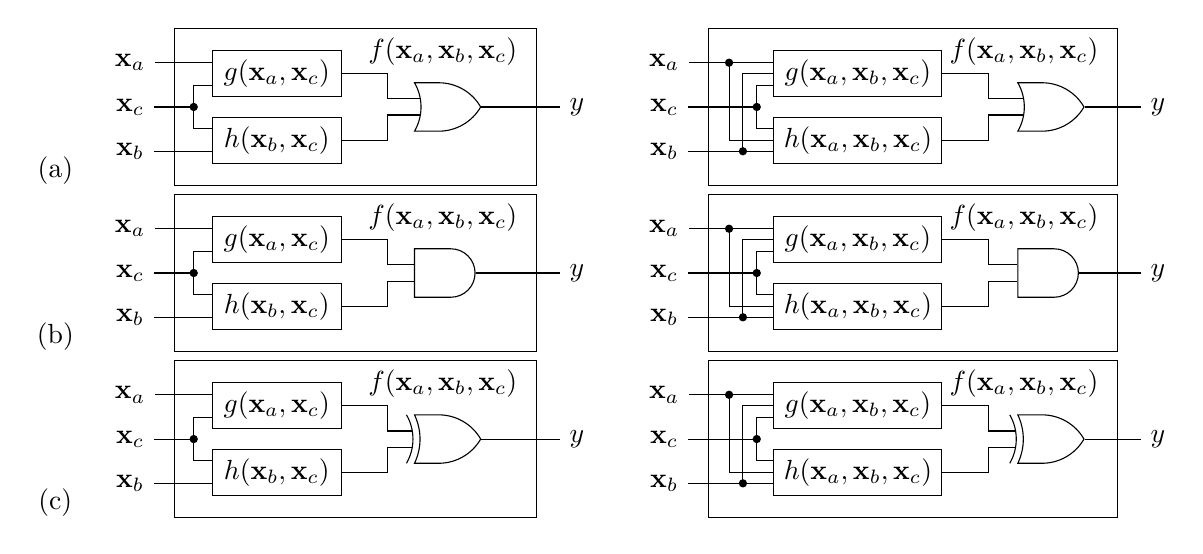
\begin{tikzpicture}[circuit logic US,
block/.style={rectangle,draw,
text width=1.4cm,
text centered,font=\sffamily,anchor=center},
block_v/.style={rectangle,draw,
text width=1.9cm,
text centered,font=\sffamily,anchor=center},
]	
\begin{scope}%[text width=1.9cm]
\node (g) [block,xshift=20, yshift=12] {$g(\bx_a,\bx_c)$};
\node (h) [block,xshift=20, yshift=-12] {$h(\bx_b,\bx_c)$};
\node (xa)[xshift=-33, yshift=16] {$\bx_a$};
\node (xc)[xshift=-33, yshift=00] {$\bx_c$};
\node (xb)[xshift=-33, yshift=-16] {$\bx_b$};
\node[cs,xshift=-10, yshift=00] (pxc) {};
\draw (-0.6,-1) -- (4,-1) -- (4,1) -- (-0.6,1) -- cycle;
\node (f) [xshift=80, yshift=20] {$f(\bx_a,\bx_b,\bx_c)$};
\node [or gate, xshift=80] (go) {}; 
\node (y)[right of=go, xshift=20] {$y$};
\draw (go.output) -- (y.west);
\draw (xa.east) -- (xa.east-|g.west);
\draw (xc.east) -- (pxc.center);
\draw (pxc.center) |- ($(g.west) + (0mm, -1.5mm)$);
\draw (pxc.center) |- ($(h.west) + (0mm, +1.5mm)$);
\draw (xb.east) -- (xb.east-|h.west);
\draw (g.east) to[--|-={5.8mm}] (go.input 1);
\draw (h.east) to[--|-={5.8mm}] (go.input 2);
\node (a) [xshift=-60, yshift=-23] {(a)};
\end{scope}
\begin{scope}[yshift=-60]
\node (g) [block,xshift=20, yshift=12] {$g(\bx_a,\bx_c)$};
\node (h) [block,xshift=20, yshift=-12] {$h(\bx_b,\bx_c)$};
\node (xa)[xshift=-33, yshift=16] {$\bx_a$};
\node (xc)[xshift=-33, yshift=00] {$\bx_c$};
\node (xb)[xshift=-33, yshift=-16] {$\bx_b$};
\node[cs,xshift=-10, yshift=00] (pxc) {};
\draw (-0.6,-1) -- (4,-1) -- (4,1) -- (-0.6,1) -- cycle;
\node (f) [xshift=80, yshift=20] {$f(\bx_a,\bx_b,\bx_c)$};
\node [and gate, xshift=80] (ga) {}; 
\node (y)[right of=ga, xshift=20] {$y$};
\draw (ga.output) -- (y.west);
\draw (xa.east) -- (xa.east-|g.west);
\draw (xc.east) -- (pxc.center);
\draw (pxc.center) |- ($(g.west) + (0mm, -1.5mm)$);
\draw (pxc.center) |- ($(h.west) + (0mm, +1.5mm)$);
\draw (xb.east) -- (xb.east-|h.west);
\draw (g.east) to[--|-={5.8mm}] (ga.input 1);
\draw (h.east) to[--|-={5.8mm}] (ga.input 2);
\node (b) [xshift=-60, yshift=-23] {(b)};
\end{scope}
\begin{scope}[yshift=-120]
\node (g) [block,xshift=20, yshift=12] {$g(\bx_a,\bx_c)$};
\node (h) [block,xshift=20, yshift=-12] {$h(\bx_b,\bx_c)$};
\node (xa)[xshift=-33, yshift=16] {$\bx_a$};
\node (xc)[xshift=-33, yshift=00] {$\bx_c$};
\node (xb)[xshift=-33, yshift=-16] {$\bx_b$};
\node[cs,xshift=-10, yshift=00] (pxc) {};
\draw (-0.6,-1) -- (4,-1) -- (4,1) -- (-0.6,1) -- cycle;
\node (f) [xshift=80, yshift=20] {$f(\bx_a,\bx_b,\bx_c)$};
\node [xor gate, xshift=80] (gxo) {}; 
\node (y)[right of=gxo, xshift=20] {$y$};
\draw (gxo.output) -- (y.west);
\draw (xa.east) -- (xa.east-|g.west);
\draw (xc.east) -- (pxc.center);
\draw (pxc.center) |- ($(g.west) + (0mm, -1.5mm)$);
\draw (pxc.center) |- ($(h.west) + (0mm, +1.5mm)$);
\draw (xb.east) -- (xb.east-|h.west);
\draw (g.east) to[--|-={5.8mm}] (gxo.input 1);
\draw (h.east) to[--|-={5.8mm}] (gxo.input 2);
\node (c) [xshift=-60, yshift=-23] {(c)};
\end{scope}
\begin{scope}[xshift=210]
\node (g) [block_v,xshift=20, yshift=12] {$g(\bx_a,\bx_b,\bx_c)$};
\node (h) [block_v,xshift=20, yshift=-12] {$h(\bx_a,\bx_b,\bx_c)$};
\node (xa)[xshift=-50, yshift=16] {$\bx_a$};
\node (xc)[xshift=-50, yshift=00] {$\bx_c$};
\node (xb)[xshift=-50, yshift=-16] {$\bx_b$};
\node[cs,xshift=-5, right of=xa] (pxa) {};
\node[cs,xshift=5, right of=xc] (pxc) {};
\node[cs,xshift=0, right of=xb] (pxb) {};
\draw (-1.2,-1) -- (4,-1) -- (4,1) -- (-1.2,1) -- cycle;
\node (f) [xshift=80, yshift=20] {$f(\bx_a,\bx_b,\bx_c)$};
\node [or gate, xshift=88] (go) {}; 
\node (y)[right of=go, xshift=12] {$y$};
\draw (go.output) -- (y.west);
\draw (xa.east) -- (xa.east-|g.west);
\draw (xc.east) -- (pxc.center);
\draw (pxa.center) |- (h.west);
\draw (pxc.center) |- ($(g.west) + (0mm, -1.5mm)$);
\draw (pxc.center) |- ($(h.west) + (0mm, +1.5mm)$);
\draw (pxb.center) |- (g.west);
\draw (xb.east) -- (xb.east-|h.west);
\draw (g.east) to[--|-={5.8mm}] (go.input 1);
\draw (h.east) to[--|-={5.8mm}] (go.input 2);
%\node (a) [xshift=-70, yshift=-23] {(a)};
\end{scope}
\begin{scope}[xshift=210,yshift=-60]
\node (g) [block_v,xshift=20, yshift=12] {$g(\bx_a,\bx_b,\bx_c)$};
\node (h) [block_v,xshift=20, yshift=-12] {$h(\bx_a,\bx_b,\bx_c)$};
\node (xa)[xshift=-50, yshift=16] {$\bx_a$};
\node (xc)[xshift=-50, yshift=00] {$\bx_c$};
\node (xb)[xshift=-50, yshift=-16] {$\bx_b$};
\node[cs,xshift=-5, right of=xa] (pxa) {};
\node[cs,xshift=5, right of=xc] (pxc) {};
\node[cs,xshift=0, right of=xb] (pxb) {};
\draw (-1.2,-1) -- (4,-1) -- (4,1) -- (-1.2,1) -- cycle;
\node (f) [xshift=80, yshift=20] {$f(\bx_a,\bx_b,\bx_c)$};
\node [and gate, xshift=88] (ga) {}; 
\node (y)[right of=ga, xshift=12] {$y$};
\draw (ga.output) -- (y.west);
\draw (xa.east) -- (xa.east-|g.west);
\draw (xc.east) -- (pxc.center);
\draw (pxa.center) |- (h.west);
\draw (pxc.center) |- ($(g.west) + (0mm, -1.5mm)$);
\draw (pxc.center) |- ($(h.west) + (0mm, +1.5mm)$);
\draw (pxb.center) |- (g.west);
\draw (xb.east) -- (xb.east-|h.west);
\draw (g.east) to[--|-={5.8mm}] (ga.input 1);
\draw (h.east) to[--|-={5.8mm}] (ga.input 2);
%\node (b) [xshift=-70, yshift=-23] {(b)};
\end{scope}
\begin{scope}[xshift=210,yshift=-120]
\node (g) [block_v,xshift=20, yshift=12] {$g(\bx_a,\bx_b,\bx_c)$};
\node (h) [block_v,xshift=20, yshift=-12] {$h(\bx_a,\bx_b,\bx_c)$};
\node (xa)[xshift=-50, yshift=16] {$\bx_a$};
\node (xc)[xshift=-50, yshift=00] {$\bx_c$};
\node (xb)[xshift=-50, yshift=-16] {$\bx_b$};
\node[cs,xshift=-5, right of=xa] (pxa) {};
\node[cs,xshift=5, right of=xc] (pxc) {};
\node[cs,xshift=0, right of=xb] (pxb) {};
\draw (-1.2,-1) -- (4,-1) -- (4,1) -- (-1.2,1) -- cycle;
\node (f) [xshift=80, yshift=20] {$f(\bx_a,\bx_b,\bx_c)$};
\node [xor gate, xshift=88] (gxo) {}; 
\node (y)[right of=gxo, xshift=12] {$y$};
\draw (gxo.output) -- (y.west);
\draw (xa.east) -- (xa.east-|g.west);
\draw (xc.east) -- (pxc.center);
\draw (pxa.center) |- (h.west);
\draw (pxc.center) |- ($(g.west) + (0mm, -1.5mm)$);
\draw (pxc.center) |- ($(h.west) + (0mm, +1.5mm)$);
\draw (pxb.center) |- (g.west);
\draw (xb.east) -- (xb.east-|h.west);
\draw (g.east) to[--|-={5.8mm}] (gxo.input 1);
\draw (h.east) to[--|-={5.8mm}] (gxo.input 2);
%\node (c) [xshift=-70, yshift=-23] {(c)};
\end{scope}
\end{tikzpicture}
	\caption{Strong bi-decompositions on the left in comparison to the vectorial bi-decomposition on the right 	
	using: 
	(a) an OR-gate; (b) an AND-gate; (c) an XOR-gate. 
	}
	\label{fig:s_v_bd}
\end{figure}

Unfortunately, there are functions for which no strong bi-decomposition exists. The completeness of the bi-decomposition provide the weak OR-bi-decomposition and the weak AND-bi-decomposition \cite{L_TQ_TKS_1989, PS_LFE_2004}. A weak XOR-bi-decomposition exists for each function, but their decomposition function can be even more complex than the given function. 

A vectorial bi-decomposition can be exist even if there is no strong bi-decomposition for a given function. Vectorial bi-decompositions were suggested in \cite{S_VBD_LF_RM_2015} for the first time. As can be seen in Figure \ref{fig:s_v_bd} on the right, vectorial bi-decompositions exist for an OR-gate, and AND-gate and also for an XOR-gate. The simplifications of the decomposition functions follow from the independence of the simultaneous change of $\bx_b$ \eqref{equ:prop_vbdg} and $\bx_a$ \eqref{equ:prop_vbdh} required in Definition \ref{def:vbd}.

\begin{definition}[Vectorial Bi-Decomposition]$\, $
\label{def:vbd}
\newline
A Boolean function $f(\bx_a,\bx_b,\bx_c)$
is OR-, AND-, or XOR-bi-decomposable with regard to the subsets of variables $\bx_a$ and $\bx_b$  
if 
\begin{enumerate}
	\item $f(\bx)$ can be expressed by
\begin{equation}
f(\bx_a,\bx_b,\bx_c)=g(\bx_a,\bx_b,\bx_c) \bullet h(\bx_a,\bx_b,\bx_c)
 \label{equ:def_vobd}
\end{equation}
where $\bullet \in \left\{ \vee, \wedge, \oplus \right\}$,
	\item the decomposition functions 
$g(\bx_a,\bx_b,\bx_c)$ and $h(\bx_a,\bx_b,\bx_c)$ satisfy 
\begin{align}
\frac{\partial g(\bx_a,\bx_b,\bx_c)}{\partial \bx_b} &= 0~,
 \label{equ:prop_vbdg}
\\
\frac{\partial h(\bx_a,\bx_b,\bx_c)}{\partial \bx_a} &= 0~.
 \label{equ:prop_vbdh}
\end{align}
\end{enumerate}
\end{definition}

\begin{example}[Vectorial bi-decomposition of a symmetric function]$\,$
\newline
The carry function $f_{c_i}(x_i,y_i,c_{i-1})$ of an adder is a symmetric function. It is known that there is no strong bi-decomposition for symmetric function. Figure \ref{fig:vsbd_cfi} shows the result of a vectorial XOR-bi-decomposition of this function. For one of the decomposition functions even exists a strong XOR-bi-decomposition, sot that the linear part of the consists of two XOR-gates.

\begin{figure}
	\centering
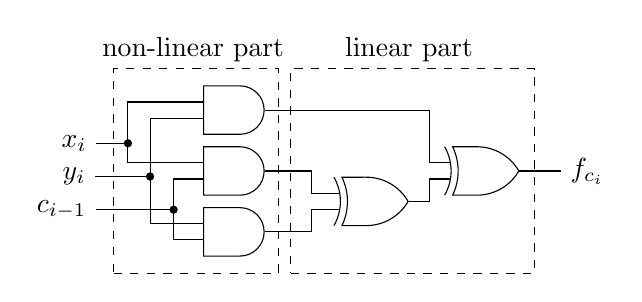
\begin{tikzpicture}[circuit logic US,
block/.style={rectangle,draw,
text width=1.6cm,
text centered,font=\sffamily,anchor=center},
]	
\begin{scope}[yshift=0]
\node (x)[xshift=-37, yshift=10] {$x_i$};
\node (y)[xshift=-37, yshift=-2] {$y_i$};
\node (c)[xshift=-41.5, yshift=-14] {$c_{i-1}$};
\node[cs,right of= x, xshift=-9 ] (px) {};
\node[cs,right of= y, xshift=-1 ] (py) {};
\node[cs,right of= c, xshift=12 ] (pc) {};
\node [and gate, xshift=20, yshift=22] (ga1) {}; 
\node [and gate, xshift=20, yshift=0] (ga2) {}; 
\node [and gate, xshift=20, yshift=-22] (ga3) {}; 
\node [xor gate, xshift=110, yshift=0] (gxo1) {}; 
\node [xor gate, xshift=70, yshift=-11] (gxo2) {}; 
\node (fci)[right of=gxo1, xshift=10] {$f_{c_i}$};
\draw (gxo1.output) -- (fci.west);
\draw (x.east) -- (px.center);
\draw (y.east) -- (py.center);
\draw (c.east) -- (pc.center);
\draw (px.center) |- (ga1.input 1);
\draw (px.center) |- (ga2.input 1);
\draw (py.center) |- (ga1.input 2);
\draw (py.center) |- (ga3.input 1);
\draw (pc.center) |- (ga2.input 2);
\draw (pc.center) |- (ga3.input 2);
\draw (ga1.output) to[--|-={20.9mm}] (gxo1.input 1);
\draw (ga2.output) to[--|-={6.0mm}] (gxo2.input 1);
\draw (ga3.output) to[--|-={6.0mm}] (gxo2.input 2);
\draw (gxo2.output) to[--|-={2.6mm}] (gxo1.input 2);
\draw[dashed] (-0.8,-1.3) -- (1.3,-1.3) -- (1.3,1.3) -- (-0.8,1.3) -- cycle;
\node [xshift=6, yshift=44] {non-linear part};
\begin{scope}[xshift=64]
\node [xshift=20, yshift=44] {linear part};
\draw[dashed] (-0.8,-1.3) -- (2.3,-1.3) -- (2.3,1.3) -- (-0.8,1.3) -- cycle;
\end{scope}
\end{scope}
\end{tikzpicture}
	\caption{Carry function $f_{c_i}(x_i,y_i,c_{i-1})$ decomposed by a vectorial EXOR-bi-decomposition followed by strong EXOR-bi-decomposition.
	}
	\label{fig:vsbd_cfi}
\end{figure}

\end{example}


\begin{table}
   \centering
        \caption{Gate equivalents for the decomposed adder}
				\vspace{6pt}
        \begin{tabular}{rrrrcc}
				\toprule
				& \multicolumn{3}{c}{Architecture on Figure \ref{fig:dec_arch}} && Standard RCA \\
                Number of Bits & Linear Part &  Nonlinear Part & Total && Total\\
                \midrule
                4  &  32     &	17	    &	49      && \phantom{1}34 \\
                5  &  65     &	39	    &	105     && \phantom{1}43 \\  
                6  &  132    &	86	    &	218     && \phantom{1}53  \\  
                7  &  266    &	180	    &	446     && \phantom{1}62  \\  
                8  &  534    &	371	    &	904     && \phantom{1}72  \\  
                10 &  2,138   &	1,520    &	3,658    && \phantom{1}91  \\  
                11 &  4,278   &	3,054	  &	7,332    && 100  \\  
                16 &  136,923 &	98,279	  &	235,202  && 148  \\  
                \bottomrule
        \end{tabular}
        \label{tab:asic_areas}
\end{table}

As it can be remarked from this table, the gate size is doubled with every bit increase. This is due to the process of internal carry generation which grows exponentially.


\begin{table}
   \centering
        \caption{Power for the decomposed adder}
				\vspace{6pt}
        %\begin{tabular}{l | c | c | c | c}
        \begin{tabular}{l  c  c  c  c}
\toprule 
           Number of Bits & Internal Power & Switching Power & Leakage Power & Total Power\\
\midrule               
                4  & 6.5159e-03 mW & 8.4444e-04 mW & 392.5974 nW & 7.7530e-03 mW\\
                5  & 1.0973e-02 mW & 1.8577e-03 mW & 822.0242 nW & 1.3653e-02 mW \\
                6  & 1.8275e-02 mW & 3.3673e-03 mW & 1.6732e+03 nW & 2.3315e-02 mW \\
                7  & 3.2342e-02 mW & 6.2124e-03 mW & 3.4077e+03 nW & 4.1962e-02 mW \\
                8  & 5.6895e-02 mW & 1.1168e-02 mW & 6.8369e+03 nW & 7.4900e-02 mW \\
                10 & 0.1868 mW  & 3.4323e-02 mW & 2.7489e+04 nW  &  0.2486 mW \\
                11 & 0.3493 mW  & 6.1830e-02 mW & 5.5015e+04 nW  &  0.4662 mW \\
                16 & 10.0527 mW & 1.6090 mW     & 1.7603e+06 nW  & 13.4228 mW\\
 \bottomrule              
        \end{tabular}
        \label{tab:asic_power}
\end{table}

\begin{table}%[!htb]
\centering
    \caption{Areas and maximal time delay for the two implementations of the decomposed adders}
		\vspace{6pt}
		\begin{tabular}{crrcrr}
\toprule
bits & \multicolumn{2}{c}{Areas (in $\unit{\mu m}$)}	&& \multicolumn{2}{c}{Time Delay (in ns)} \\
\cmidrule{2-3}
\cmidrule{5-6} 
  & Global & Local && Global & Local \\
\midrule 
4	 & 70 & 49 && 0.62 & 0.70 \\ 
5	 & 150 & 68 && 1.00 & 0.97 \\ 
6	 & 314 & 87 && 1.69 & 1.24 \\ 
7	 & 643 & 105 && 3.24 & 1.50 \\ 
8	 & 1,302 & 124 && 5.97 & 1.77 \\ 
9	 & 2,623 & 143 && 11.38 & 2.03 \\ 
10	 & 5,268 & 162 && 22.25 & 2.30 \\ 
11	 & 10,558 & 180 && 43.75 & 2.56 \\ 
16	 & 338,690 & 274 && 1379.43 & 3.89 \\ 
\bottomrule
\end{tabular}
   \label{tab:cla_vs_rca_area_timing}
\end{table}

\section{Experimental Results - ASIC and FPGA Synthesis}

Due the results of Subsection \ref{subsec:lin_wrt_v} we compare two synthesis approaches. The first one uses the 
architecture shown in Figure \ref{fig:dec_arch} for complete adders of different numbers of bits (similar to a carry look-ahead adder (CLA)). The second one uses vectorial and strong bi-decompositions as shown in Figure~\ref{fig:vsbd_cfi} for adders with a restricted number of bits and generates larger adders in an architecture similar to a ripple carry adder (RCA). In both architectures we assume that there is no carry in and carry out.

\subsection{ASIC  Synthesis}

The adders were synthesized in 65nm CMOS technology using the Design Compiler from Synopsys. 
The global decomposition results in very large area of implementation as noted in Table~\ref{tab:asic_areas}.
Table~\ref{tab:asic_power} shows the power associated to implementations on ASIC of the globally decomposed adder for different number of bits. 



Table~\ref{tab:cla_vs_rca_area_timing} compares both the area and the maximum delay for the two different implementations of the decomposed adder.
We can see that the local decomposition results in much smaller area.
Moreover, the maximum delay in the local decomposition is significantly shorter.
For these reasons the FPGA synthesis was then done only for the locally decomposed adder.



\subsection{FPGA Synthesis}
Tables~\ref{tab:fpga_area}, \ref{tab:fpga_power} and \ref{tab:fpga_timing} show the area, power, and timing  associated to implementations on FPGA of the decomposed adder for different number of bits and compares them to the equivalent values for a standard adder. 
Synthesis and routing was done for a Zynq FPGA using the Vivado design suite.


\begin{table}%[htb]
	\centering
	\caption{Number of LUTs used}
\vspace{6pt}		
		\begin{tabular}{cccp{4mm}ccc}
\toprule		
bits & decomposed & undecomposed & & bits & decomposed & undecomposed \\
\cmidrule{1-3}
\cmidrule{5-7}
4  &  4 &  4 & & 19 & 20 & 19 \\
5  &  4 &  4 & & 20 & 21 & 20 \\
6  &  6 &  6 & & 21 & 22 & 21 \\
7  &  6 &  7 & & 22 & 23 & 22 \\
8  &  8 &  8 & & 23 & 24 & 23 \\
9  &  8 &  9 & & 24 & 25 & 24 \\
10 & 10 & 10 & & 25 & 26 & 25 \\
11 & 10 & 11 & & 26 & 27 & 26 \\
16 & 42 & 16 & & 31 & 32 & 31 \\
\bottomrule
		\end{tabular}
    \label{tab:fpga_area}
\end{table}


\begin{table}%[ht]
\centering
    \caption{Power}
		\vspace{6pt}
    \begin{tabular}{ccccccc}
		\toprule
    bits	 & decomposed	 & standard && bits	 & decomposed	 & standard\\ 
    \cmidrule{1-3}\cmidrule{5-7} 
    4	 & 2.399	 & 2.399 && 19	 & 13.283	 & 14.187 \\ 
    5	 & 3.068	 & 3.068 && 20	 & 13.936	 & 14.922  \\ 
    6	 & 3.741	 & 4.054 && 21	 & 14.610	 & 15.655 \\ 
    7	 & 4.432	 & 4.813 && 22	 & 15.272	 & 16.388 \\ 
    8	 & 5.134	 & 5.591 && 23	 & 15.942	 & 17.119\\ 
    9	 & 5.847	 & 6.395 && 24	 & 16.631	 & 17.857  \\ 
    10	 & 6.583	 & 7.226 && 25	 & 17.285	 & 18.564 \\ 
    11	 & 7.347	 & 8.105 && 26	 & 17.745	 & 19.202 \\ 
    12	 & 8.153	 & 8.974 && 27	 & 18.427	 & 19.951 \\ 
    13	 & 8.945	 & 9.702 && 28	 & 19.081	 & 20.701 \\ 
    14	 & 12.222	 & 10.441 && 29	 & 19.734	 & 21.465 \\ 
    15	 & 13.159	 & 11.172 && 30	 & 20.412	 & 22.212 \\ 
    16	 & 14.021	 & 11.909 && 31	 & 21.104	 & 22.957 \\ 
    17	 & 15.241	 & 12.739 && 32	 & 21.784	 & 23.727 \\ 
    18	 & 16.092	 & 13.470   \\ 
		\bottomrule
    \end{tabular}
    \label{tab:fpga_power}
\end{table}

\begin{table}%[htb]
\centering
    \caption{Timing (max delay path in ns)}
		\vspace{6pt}
   \begin{tabular}{ccccccc}
		\toprule
    bits	 & decomposed	 & standard && bits	 & decomposed	 & standard \\ 
    \cmidrule{1-3}\cmidrule{5-7} 
    4	 & 7.875	 & 7.875 && 19	 & 26.894	 & 10.306  \\ 
    5	 & 8.321	 & 8.321 && 20	 & 26.327	 & 10.052  \\ 
    6	 & 8.278	 & 8.348 && 21	 & 28.798	 & 10.252  \\ 
    7	 & 8.729	 & 8.371 && 22	 & 30.979	 & 10.518  \\ 
    8	 & 9.074	 & 8.689 && 23	 & 31.079	 & 10.506  \\ 
    9	 & 10.462	 & 8.518 && 24	 & 31.556	 & 10.52 \\ 
    10	 & 10.707	 & 8.958 && 25	 & 35.130	 & 10.212 \\ 
    11	 & 12.007	 & 8.956 && 26	 & 34.476	 & 10.634 \\ 
    12	 & 12.258	 & 9.082 && 27	 & 34.620	 & 10.628 \\ 
    13	 & 13.345	 & 8.903 && 28	 & 36.111	 & 10.865 \\ 
    14	 & 18.462	 & 9.162 && 29	 & 33.641	 & 10.739 \\ 
    15	 & 19.567	 & 9.427 && 30	 & 38.501	 & 10.847 \\ 
    16	 & 19.486	 & 9.578 && 31	 & 39.772	 & 11.074 \\ 
    17	 & 21.299	 & 9.911 && 32	 & 40.908	 & 11.203 \\ 
    18	 & 22.309	 & 10.052 &&  \\ 
\bottomrule
    \end{tabular}
    \label{tab:fpga_timing}
\end{table}

While for the locally decomposed adder the number of gates and associated delay is drastically improved, one needs to consider further optimization for the circuits such that the presented architectures become competitive. For the locally decomposed adder a particular emphasis will be on implementations on FPGA and power optimization. Further study into using academic tools for logic synthesis and optimization such as Expresso, SIS, ABC, etc. will be also performed. 


\chapter{CPE}

\chapter{Integration} %linear+cpe

\chapter{Results}

\chapter{Conclusions}

With the continuing logic technology scaling, design for reliability/power/test is becoming a major concern. In this context, a significant effort across recent years was in efficient decomposition of logic functions in AND/XOR or OR/XOR networks.
The strong EXOR-bi-decomposition is an alternative method to split a
give Boolean function into simpler decomposition function using an EXOR-gate.
The vectorial bi-decomposition extents the possibilities for decomposition. We show that even in
the case of the symmetric carry function, for which no strong bi-decomposition
exists, a decomposition into a linear output-part and a non-linear input part
could be designed. A Reed-Muller form for the adder can be achieved. Also, some quantification in terms of degree of linearization is given. Using the proposed decomposition, we implement the resulting decomposed adders on ASIC and FPGA technologies and give some preliminary results. The results show that further development of custom optimization tools is required. This is part of future work together with the integration of code prediction encoding for improved reliability.


\bibliographystyle{plain}
\bibliography{bib_popovici,bib_steinbach}

\end{document}
